\documentclass[aspectratio=169]{beamer}

% --- Theme Configuration ---
\usetheme{Madrid}
\usecolortheme{whale} % Dark blue aesthetic
\setbeamercolor{titlelike}{parent=structure,bg=blue!80!black,fg=white}

% --- Packages ---
\usepackage{graphicx}
\usepackage{booktabs}
\usepackage{hyperref}
\usepackage{tikz}
\usepackage{tcolorbox}

% --- Title Information ---
\title[Instrunet AI]{INSTRUNET AI}
\subtitle{Deep Learning for Music Instrument Recognition}
\author{Jagath Kiran}
\date{January 21, 2026}

\begin{document}

% 1. Title Slide
\begin{frame}[plain]
    \titlepage
\end{frame}

% 2. Table of Contents
\begin{frame}{TABLE OF CONTENTS}
    \begin{columns}
        \column{0.6\textwidth}
        \begin{itemize}
            \item PROJECT OVERVIEW
            \item DATASET OVERVIEW AND KEY INSIGHTS
            \item METHODOLOGY
            \item DATA PREPROCESSING
            \item FEATURE EXTRACTION
            \item MODEL ARCHITECTURE
            \item TRAINING AND EVALUATION
            \item RESULTS
            \item USER INTERFACE
            \item CHALLENGES
            \item FUTURE SCOPE
            \item CONCLUSION
        \end{itemize}
        \column{0.4\textwidth}
        \centering
        \includegraphics[width=0.8\textwidth]{../../outputs/frontend/dashboard_audio_spectrogram.png}
    \end{columns}
\end{frame}

% 3. Project Overview
\section{PROJECT OVERVIEW}
\begin{frame}{PROJECT OVERVIEW}
    \begin{block}{OBJECTIVE:}
        To build a model that can automatically identify the predominant musical instrument in a given audio track. Instrument identification is essential for music information retrieval, automatic transcription, and intelligent music recommendation systems.
    \end{block}
    
    \begin{block}{OUTCOMES:}
        \begin{itemize}
            \item A trained deep learning model capable of predicting the instrument class of input audio with high precision.
            \item Improved robustness in detection across varied recording conditions using advanced data augmentation.
        \end{itemize}
    \end{block}
\end{frame}

% 4. Dataset Overview
\section{DATASET OVERVIEW}
\begin{frame}{DATASET OVERVIEW AND KEY INSIGHTS}
    \begin{columns}
        \column{0.5\textwidth}
        \textbf{Structure:} Audio tracks (WAV/MP3) with label files.\\
        \textbf{Size:} ~6,700 samples (IRMAS Training) + NSynth Secondary.\\
        \textbf{Strengths:} High-quality studio recordings and diverse instrument classes.
        
        \column{0.5\textwidth}
        \textbf{REASON OF CHOOSING THE DATASET:}
        \begin{itemize}
            \item \textbf{Rich Timbral Variety:} Covers 11 distinct classes including strings, winds, and percussion.
            \item \textbf{Industry Standard:} IRMAS is a widely recognized benchmark for instrument recognition.
            \item \textbf{Scalable:} Foundation for moving toward multi-label polyphonic detection.
        \end{itemize}
    \end{columns}
\end{frame}

% 5. Methodology
\section{METHODOLOGY}
\begin{frame}{METHODOLOGY}
    \begin{itemize}
        \item \textbf{DATA PREPROCESSING:} Cleaning, resampling, and windowing raw audio signals.
        \item \textbf{FEATURE EXTRACTION:} Converting time-domain audio into frequency-domain RGB Spectrograms.
        \item \textbf{MODEL ARCHITECTURE:} Designing a custom CNN optimized for harmonic texture analysis.
        \item \textbf{TRAINING AND EVALUATION:} Iterative optimization using SpecAugment and performance benchmarking.
    \end{itemize}
    \vspace{0.5cm}
    \centering
    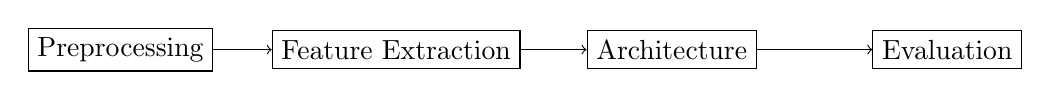
\begin{tikzpicture}[node distance=2cm, auto]
        \node [draw, rectangle] (p1) {Preprocessing};
        \node [draw, rectangle, right of=p1, xshift=1.5cm] (p2) {Feature Extraction};
        \node [draw, rectangle, right of=p2, xshift=1.5cm] (p3) {Architecture};
        \node [draw, rectangle, right of=p3, xshift=1.5cm] (p4) {Evaluation};
        \draw [->] (p1) -- (p2);
        \draw [->] (p2) -- (p3);
        \draw [->] (p3) -- (p4);
    \end{tikzpicture}
\end{frame}

% 6. Data Preprocessing
\section{DATA PREPROCESSING}
\begin{frame}{Data Preprocessing}
    \begin{enumerate}
        \item \textbf{RESAMPLING \& MONO CONVERSION:} All audio is standardized to 22.05 kHz and converted to mono to ensure consistent feature dimensions.
        \item \textbf{WINDOWING:} Longer tracks are sliced into 3-second segments with 50\% overlap to capture temporal variations in timbre.
        \item \textbf{SILENCE REMOVAL:} Low-energy segments are filtered out to prevent the model from learning "noise" or "silence" as features.
    \end{enumerate}
\end{frame}

% 7. Feature Extraction
\section{FEATURE EXTRACTION}
\begin{frame}{Feature Extraction}
    \begin{enumerate}
        \item \textbf{MEL-SPECTROGRAM GENERATION:} Applying Short-Time Fourier Transform (STFT) mapped to the Mel scale, which mimics human auditory perception.
        \item \textbf{LOG-AMPLITUDE SCALING:} Converting power to decibels (dB) to highlight harmonic structures over a wide dynamic range.
        \item \textbf{NORMALIZATION:} Rescaling pixel values to [0, 1] and resizing to \textbf{224x224} RGB images for compatibility with deep learning backbones.
    \end{enumerate}
\end{frame}

% 8. Model Architecture
\section{MODEL ARCHITECTURE}
\begin{frame}{Model Architecture}
    \begin{columns}
        \column{0.6\textwidth}
        The architecture is a deep Convolutional Neural Network (CNN) built for high-dimensional texture analysis.
        \begin{itemize}
            \item \textbf{CONV BLOCKS:} 4 stages (32, 64, 128, 256 filters) with Batch Normalization.
            \item \textbf{REGULARIZATION:} Spatial Dropout (0.5) and L2 Regularization to prevent overfitting.
            \item \textbf{POOLING:} Global Average Pooling to ensure shift-invariance.
            \item \textbf{OUTPUT:} 11-way Softmax for single-instrument classification.
        \end{itemize}
        \column{0.4\textwidth}
        \begin{figure}
            \centering
            \includegraphics[width=\textwidth]{../../outputs/training_history.png}
            \caption{Learning Curves}
        \end{figure}
    \end{columns}
\end{frame}

% 9. Training and Evaluation
\section{TRAINING AND EVALUATION}
\begin{frame}{Training and Evaluation}
    The dataset was divided into 80\% for training and 20\% for validation, ensuring no data leakage via "Split-First" augmentation.
    
    \vspace{0.3cm}
    \begin{table}[]
        \centering
        \begin{tabular}{lcccc}
            \toprule
            \textbf{Metric} & \textbf{Precision} & \textbf{Recall} & \textbf{F1-Score} \\
            \midrule
            Overall Accuracy & - & - & \textbf{82.24\%} \\
            Macro Average & 0.81 & 0.82 & 0.81 \\
            Weighted Average & 0.82 & 0.82 & 0.82 \\
            \bottomrule
        \end{tabular}
    \end{table}
    
    \textbf{SpecAugment Performance:} Integrating Time and Frequency masking reduced high-confidence errors and improved generalization.
\end{frame}

% 10. Results
\section{RESULTS}
\begin{frame}{Results}
    \begin{columns}
        \column{0.5\textwidth}
        \begin{itemize}
            \item \textbf{BEST PERFORMERS:} Voice (0.92 F1) and Organ (0.92 F1). The model identifies harmonic stacks with near-perfect reliability.
            \item \textbf{CHALLENGES:} Violin and Saxophone (0.71 F1) show timbral overlap with Cello and Trumpet.
            \item \textbf{ROBUSTNESS:} ROC-AUC scores indicate excellent class separation.
        \end{itemize}
        \column{0.5\textwidth}
        \begin{figure}
            \centering
            \includegraphics[width=0.8\textwidth]{../../outputs/normalized_confusion_matrix.png}
        \end{figure}
    \end{columns}
\end{frame}

% 11. User Interface
\section{USER INTERFACE}
\begin{frame}{USER INTERFACE}
    \begin{columns}
        \column{0.5\textwidth}
        \begin{figure}
            \centering
            \includegraphics[width=\textwidth]{../../outputs/frontend/login_page.png}
            \caption{Secure Login Portal}
        \end{figure}
        \column{0.5\textwidth}
        \begin{figure}
            \centering
            \includegraphics[width=\textwidth]{../../outputs/frontend/dashboard_predictions.png}
            \caption{Live Analysis Dashboard}
        \end{figure}
    \end{columns}
\end{frame}

% 12. Challenges
\section{CHALLENGES}
\begin{frame}{Challenges}
    \begin{enumerate}
        \item \textbf{DATA IMBALANCE:} Handled via class-weighting during training to ensure rare instruments (like Flute) are not ignored.
        \item \textbf{TIMBRAL OVERLAP:} Disentangling similar harmonic signatures (e.g., Bowed strings vs. Woodwinds) required higher input resolutions (224x224).
        \item \textbf{ENVIRONMENT MISMATCH:} Bridging the gap between studio training data and real-world noisy audio uploads.
    \end{enumerate}
\end{frame}

% 13. Future Scope
\section{FUTURE SCOPE}
\begin{frame}{Future Scope}
    \begin{columns}
        \column{0.6\textwidth}
        \begin{itemize}
            \item \textbf{PERSISTENCE:} Integrating Supabase for cloud-based report storage and user history.
            \item \textbf{POLYPHONY:} Retraining with Multi-Label heads (Sigmoid) to detect multiple instruments playing simultaneously.
            \item \textbf{ATTENTION:} Implementing Transformer-based backbones (AST) for global spectral context.
        \end{itemize}
        \column{0.4\textwidth}
        \begin{figure}
            \centering
            \includegraphics[width=\textwidth]{../../outputs/roc_curves.png}
        \end{figure}
    \end{columns}
\end{frame}

% 14. Conclusion
\section{CONCLUSION}
\begin{frame}{CONCLUSION}
    \begin{itemize}
        \item Successfully developed a deep learning system for accurate instrument detection with \textbf{82.2\% accuracy}.
        \item Achieved robust performance across 11 classes using custom CNN architectures and SpecAugment.
        \item Demonstrated the feasibility of real-time audio analysis through a deployed full-stack web application.
    \end{itemize}
\end{frame}

% 15. Thank You
\begin{frame}[plain]
    \centering
    \Huge{THANK YOU}
\end{frame}

\end{document}
